\documentclass[UTF8,a4paper,12pt]{ctexart}

\usepackage[margin=2cm]{geometry}
\usepackage{amsmath,amssymb}
\usepackage{graphicx}
\graphicspath{{figures/}}
\usepackage{caption}
\usepackage{subcaption}
\usepackage{booktabs}
\usepackage{array}
\usepackage{float}
\usepackage{xcolor}
\usepackage{listings}
\usepackage{tikz}
\usetikzlibrary{arrows.meta,positioning,calc}
\usepackage{zhnumber}
\usepackage{hyperref}

\hypersetup{
  colorlinks=true,
  linkcolor=black,
  urlcolor=blue
}

\captionsetup{font=small,labelfont=bf}
\setlength{\parindent}{2em}
\setlength{\parskip}{0.25em}
\renewcommand{\arraystretch}{1.18}

\lstdefinestyle{cppstyle}{
  language=C++,
  basicstyle=\ttfamily\small,
  keywordstyle=\color{blue!65!black}\bfseries,
  commentstyle=\color{green!35!black},
  stringstyle=\color{red!55!black},
  numbers=left,
  numberstyle=\tiny\color{gray},
  stepnumber=1,
  numbersep=8pt,
  frame=single,
  rulecolor=\color{black!35},
  breaklines=true,
  columns=fullflexible,
  keepspaces=true,
  showstringspaces=false,
  tabsize=2
}
\lstset{style=cppstyle}

\newcounter{makepart}
\setcounter{makepart}{1}
\NewDocumentCommand{\makepart}{+m}
{
  \vspace{0.8em}
  \begin{flushleft}
   \large\bfseries\zhnumber{\arabic{makepart}}、#1
  \end{flushleft}
  \stepcounter{makepart}
}

\NewDocumentCommand{\zdx}{}
{
  \tikz[remember picture,overlay]{
    \coordinate (s) at ([shift={(1,-3)}]current page.north west);
    \coordinate (e) at ([shift={(1,3)}]current page.south west);
    \foreach \x in{0,0.15,...,9.2}
    {
      \fill[] ($(s)+(0,-\x)$) circle(1pt);
    }
    \foreach \x in{0,0.15,...,9.2}
    {
      \fill[] ($(e)+(0,\x)$) circle(1pt);
    }
    \node[text width=1em,align=center] at ($(s)!0.5!(e)$) {装\\[10pt]订\\[10pt]线};
  }
}

\NewDocumentCommand{\makecoveri}{}
{
  \thispagestyle{empty}
  \noindent\begin{minipage}[c][170pt][c]{\textwidth}
    {\Large\bfseries 电子电路设计实验 II\par}
    \vspace{14pt}
    {\LARGE\bfseries 倒计时定时器实验报告\par}
  \end{minipage}\par\vspace{12pt}
}

\begin{document}
\makecoveri

\makepart{实验目的}

本实验围绕基于 Arduino UNO 的倒计时定时器扩展板展开，目标是完成从需求分析、原理图设计、PCB 绘制到程序调试的完整工程流程。实验要求定时器能够通过旋转编码器选择预设倒计时时间，在四位 7 段数码管上显示分钟和秒，并在倒计时结束后由蜂鸣器给出声响提示。通过本设计，可掌握旋转编码器输入、共阴极数码管动态扫描、蜂鸣器功率驱动、EEPROM 掉电存储以及 Arduino UNO 扩展板 PCB 设计等关键内容。

结合参考资料中的基础方案，本次设计特别强调两点：其一，显示部分不沿用参考程序中的共阳极逻辑，而是按照实验要求采用共阴极（Common Cathode）两位 7 段 LED 数码管；其二，在蜂鸣器报警支路中增加三极管 Q0，使 Arduino I/O 口不直接承受蜂鸣器工作电流，提高驱动裕量与接口可靠性。

\makepart{实验任务与技术指标}

本项目的功能指标如表 \ref{tab:requirements} 所示。定时器工作状态分为停止设定状态和倒计时运行状态：停止状态下旋转编码器用于选择标准时间数组中的时间，按下编码器开关后进入运行状态；运行状态下系统以 $1\,\mathrm{s}$ 为基本节拍递减显示时间，计时结束时触发蜂鸣器报警；再次按下编码器开关可切换状态并关闭报警输出。

\begin{table}[H]
  \centering
  \caption{A4 倒计时定时器功能指标与实现方式}
  \label{tab:requirements}
  \begin{tabular}{>{\raggedright\arraybackslash}p{0.16\textwidth}
                  >{\raggedright\arraybackslash}p{0.34\textwidth}
                  >{\raggedright\arraybackslash}p{0.38\textwidth}}
    \toprule
    指标类别 & 设计要求 & 本设计实现方式 \\
    \midrule
    主控平台 & Arduino UNO 兼容扩展板 & U1 采用 Arduino-UNO-EX 引脚排布 \\
    时间设定 & 可选择若干倒计时时间 & 旋转编码器选择标准时间数组索引 \\
    显示方式 & 显示分钟、秒 & 两片共阴极 2 位 7 段 LED，动态扫描 \\
    报警方式 & 时间到达后声音提示 & D11 经 R0 驱动 NPN 三极管 Q0 控制蜂鸣器 \\
    掉电记忆 & 上电恢复上次设定 & EEPROM 保存 selectedTimeIndex \\
    PCB 实现 & 完成扩展板焊接与联调 & 制板原理图、PCB 版图、焊接实物与上电测试 \\
    \bottomrule
  \end{tabular}
\end{table}

\makepart{系统总体方案与需求分析}

系统的信号流如图 \ref{fig:system-block} 所示。旋转编码器输出 A、B 两相脉冲以及按键电平，Arduino UNO 读取输入状态后进行时间索引更新、状态切换和倒计时运算；显示支路由段选信号与位选信号共同完成四位数码管动态扫描；报警支路由 I/O 口控制三极管开关，再驱动蜂鸣器；EEPROM 用于保存最后一次选择的时间索引，使系统断电后仍可恢复常用设定。

\begin{figure}[H]
  \centering
  \begin{tikzpicture}[
    block/.style={draw, rounded corners=2pt, text width=3.05cm, minimum height=1.18cm, align=center, fill=gray!8, font=\small},
    main/.style={draw, rounded corners=2pt, text width=3.05cm, minimum height=1.42cm, align=center, fill=blue!6, font=\small},
    arr/.style={-{Stealth[length=2.5mm]}, thick, shorten >=2pt, shorten <=2pt},
    lab/.style={fill=white, inner sep=1pt, font=\small}
  ]
    \node[block] at (0,0) (enc) {旋转编码器\\A/B 相与按键};
    \node[main] at (5.0,0) (mcu) {Arduino UNO\\状态控制与计时};
    \node[block] at (10.0,0) (disp) {共阴极数码管\\段选 + 位选\\动态扫描};
    \node[block] at (5.0,-2.55) (eeprom) {EEPROM\\保存时间索引};
    \node[block] at (10.0,-2.55) (buzz) {蜂鸣器报警\\Q0 开关驱动};
    \draw[arr] (enc) -- node[lab, above, midway]{输入检测} (mcu);
    \draw[arr] (mcu) -- node[lab, above, midway]{显示数据} (disp);
    \draw[arr] (mcu.south) -- node[lab, left, midway]{读写} (eeprom.north);
    \draw[arr] (mcu.south east) -- node[lab, above right, pos=0.55]{报警控制} (buzz.north west);
  \end{tikzpicture}
  \caption{A4 倒计时定时器系统框图与主要信号流}
  \label{fig:system-block}
\end{figure}

从资源分配看，四位 7 段显示若采用静态驱动，需要约 $4\times8=32$ 根段控制线，远超 Arduino UNO 直接 I/O 资源的舒适范围。因此本设计采用动态扫描方式：同名段线并联作为段选，四个公共阴极分别由位选三极管控制，使显示 I/O 数量降至 8 根段选线加 4 根位选线。设刷新周期为 $T_s$，四位数码管单次点亮时间约为 $T_s/4$。当刷新频率满足
\begin{equation}
  f_s=\frac{1}{T_s}\geq 100\,\mathrm{Hz}
  \label{eq:scan-frequency}
\end{equation}
时，每位的重复点亮频率足以利用人眼视觉暂留形成稳定显示。式 \eqref{eq:scan-frequency} 中 $f_s$ 为完整四位扫描频率，单位为赫兹。

\makepart{硬件电路设计与优化}

\subsection*{1. 显示模块设计}

参考资料说明 7 段数码管可分为共阳极和共阴极两类。实验要求明确指出，参考例程中的数码管为共阳设计，而本项目应按共阴极情况设计。因此，本设计选用两片 HDSM-577G 型 2 位共阴极 7 段 LED，构成 MMSS 四位显示。其结构和封装引脚如图 \ref{fig:segment-package} 所示。

\begin{figure}[H]
  \centering
  \begin{subfigure}[t]{0.48\textwidth}
    \centering
    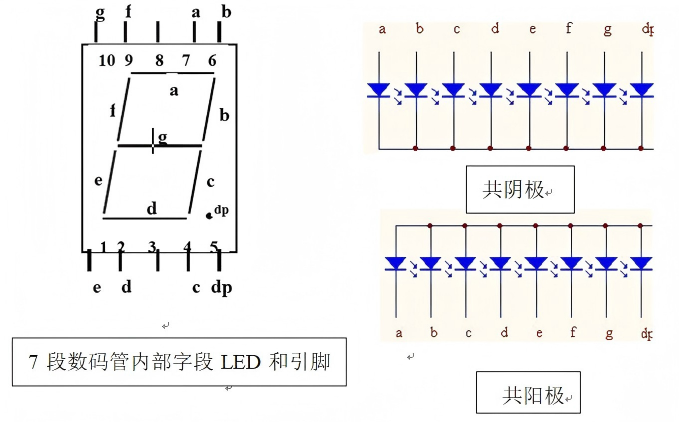
\includegraphics[width=0.95\linewidth]{seven_segment_structure.png}
    \caption{7 段数码管发光段结构}
    \label{fig:segment-structure}
  \end{subfigure}
  \hfill
  \begin{subfigure}[t]{0.48\textwidth}
    \centering
    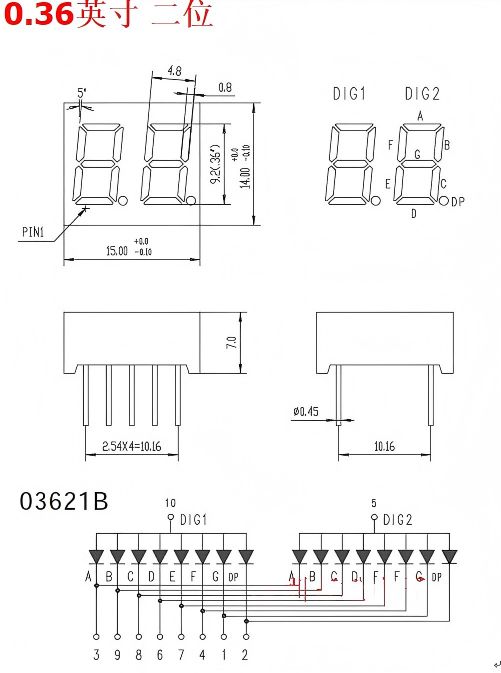
\includegraphics[width=0.72\linewidth]{dual_digit_package.png}
    \caption{2 位共阴极 LED 封装与引脚}
    \label{fig:dual-package}
  \end{subfigure}
  \caption{A4 倒计时定时器显示器件结构与封装信息}
  \label{fig:segment-package}
\end{figure}

在共阴极驱动条件下，某一位数码管被选通时，其公共阴极经对应的 NPN 三极管接近地电位；同时 Arduino 在需要点亮的段线上输出高电平，段电流从 I/O 口经限流电阻、LED 段流入位选三极管并回到地。以单段 LED 正向压降 $V_F$、段限流电阻 $R_{\mathrm{seg}}$、三极管饱和压降 $V_{CE(\mathrm{sat})}$ 表示，单段峰值电流近似为
\begin{equation}
  I_{\mathrm{seg}}=\frac{V_{CC}-V_F-V_{CE(\mathrm{sat})}}{R_{\mathrm{seg}}}.
  \label{eq:segment-current}
\end{equation}
其中 $V_{CC}=5\,\mathrm{V}$，$R_{\mathrm{seg}}=100\,\Omega$。若取绿色 LED 的典型 $V_F\approx2.1\,\mathrm{V}$、小功率 NPN 饱和压降 $V_{CE(\mathrm{sat})}\approx0.2\,\mathrm{V}$，则 $I_{\mathrm{seg}}\approx27\,\mathrm{mA}$。由于动态扫描中每位占空比约为 $1/4$，单段平均电流约为峰值电流的四分之一，可在亮度与 Arduino 引脚能力之间取得折中。实际调试时应结合数码管亮度、I/O 总电流限制和发热情况必要时增大段电阻。

图 \ref{fig:schematic} 给出了本次设计的完整原理图。D3、D2、D19、D16、D18、D4、D5、D17 经 $100\,\Omega$ 电阻分别连接 a、b、c、d、e、f、g、dp 段线；D14、D7、D15、D6 通过 Q1--Q4 控制四个公共阴极，实现分时位选。共阴极逻辑下，段选为高电平有效，位选三极管基极为高电平时对应数码管被选通，这与共阳极参考程序中“段码取反”的写法不同，软件必须同步调整。

\begin{figure}[H]
  \centering
  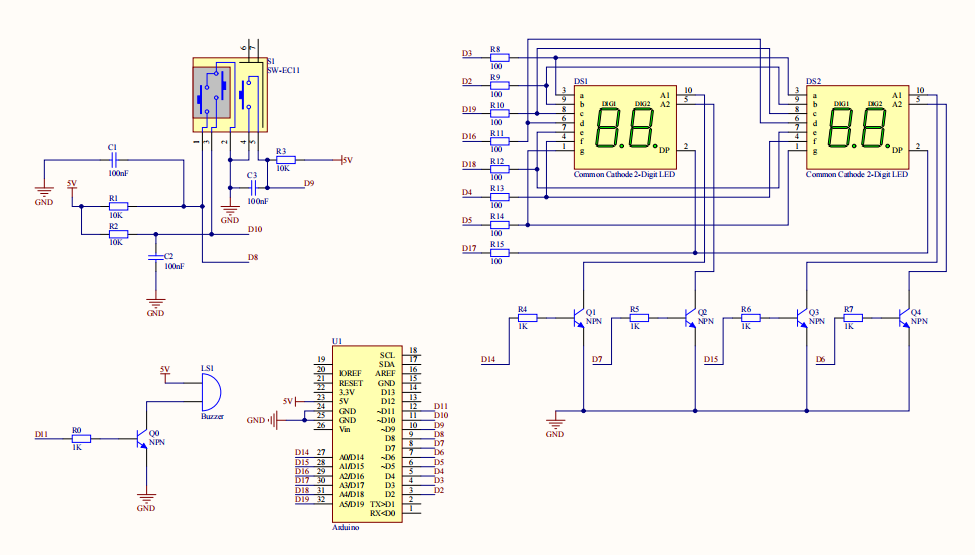
\includegraphics[width=0.98\textwidth]{schematic.png}
  \caption{A4 倒计时定时器共阴极显示与报警驱动完整原理图}
  \label{fig:schematic}
\end{figure}

\subsection*{2. 报警驱动电路优化}

基础参考电路中蜂鸣器可由 Arduino 输出口直接控制，但这种连接方式要求 I/O 口直接承担蜂鸣器工作电流，若蜂鸣器启动电流或持续电流偏大，可能造成端口电压下陷、发声不稳定甚至损伤单片机端口。本设计在蜂鸣器 LS1 支路加入 NPN 三极管 Q0，如图 \ref{fig:schematic} 左下角所示：LS1 一端接 $5\,\mathrm{V}$，另一端接 Q0 集电极，Q0 发射极接地，D11 经基极电阻 R0 接入 Q0 基极。

Q0 在该处作为低端开关管使用，其状态可表示为
\begin{equation}
  Q0=
  \begin{cases}
    \text{截止，蜂鸣器不响}, & V_{D11}\approx0\,\mathrm{V},\\
    \text{饱和导通，蜂鸣器响}, & V_{D11}\approx5\,\mathrm{V}.
  \end{cases}
  \label{eq:q0-state}
\end{equation}
当 D11 输出低电平时，基极-发射极结未正向偏置，$I_B\approx0$，集电极电流被切断；当 D11 输出高电平时，基极电流约为
\begin{equation}
  I_B=\frac{V_{OH}-V_{BE}}{R_0}
  \approx \frac{5.0\,\mathrm{V}-0.7\,\mathrm{V}}{1\,\mathrm{k}\Omega}
  =4.3\,\mathrm{mA}.
  \label{eq:base-current}
\end{equation}
在强迫电流放大倍数按 $\beta_{\mathrm{forced}}\approx10$ 估算时，Q0 可提供约 $40\,\mathrm{mA}$ 量级的集电极驱动裕量。由此，Arduino D11 仅提供基极电流，蜂鸣器主电流由 $5\,\mathrm{V}$ 电源经 Q0 承担，实现了驱动电流放大和 I/O 口隔离保护。对于电磁式蜂鸣器，进一步工程优化可在蜂鸣器两端并联续流二极管，以抑制断开瞬间的感性反冲；若使用有源压电蜂鸣器，则 Q0 开关驱动已能满足基本报警需求。

\subsection*{3. 输入模块设计}

旋转编码器 S1 具有 A、B 两相输出和一个按压开关。旋钮旋转时，A 相和 B 相输出近似正交的方波序列；顺时针与逆时针旋转时，两个相位的先后关系相反。设在 A 相下降沿采样 B 相电平，则可用表 \ref{tab:encoder} 判定旋转方向。原理图中 R1、R2 为上拉电阻，C1、C2 形成输入端低通滤波；按键支路由 R3 上拉，C3 抑制机械按键抖动。

\begin{table}[H]
  \centering
  \caption{旋转编码器 A 相下降沿方向判定逻辑}
  \label{tab:encoder}
  \begin{tabular}{>{\raggedright\arraybackslash}p{0.16\textwidth}
                  >{\raggedright\arraybackslash}p{0.34\textwidth}
                  >{\raggedright\arraybackslash}p{0.38\textwidth}}
    \toprule
    检测事件 & B 相采样状态 & 软件返回值 \\
    \midrule
    A 相由高到低 & B 为高电平 & $-1$ 或逆时针步进 \\
    A 相由高到低 & B 为低电平 & $+1$ 或顺时针步进 \\
    A、B 无有效变化 & 任意 & $0$ \\
    \bottomrule
  \end{tabular}
\end{table}

\subsection*{4. 元器件选型与功能分组}

元器件清单图片如图 \ref{fig:bom-image} 所示。为避免只按编号罗列，表 \ref{tab:bom} 按功能模块对关键器件进行归纳。显示支路中 $100\,\Omega$ 段电阻用于限制 LED 峰值电流；Q1--Q4 承担位选电流汇流；Q0 专门承担蜂鸣器电流，避免 D11 直接驱动负载。

\begin{figure}[H]
  \centering
  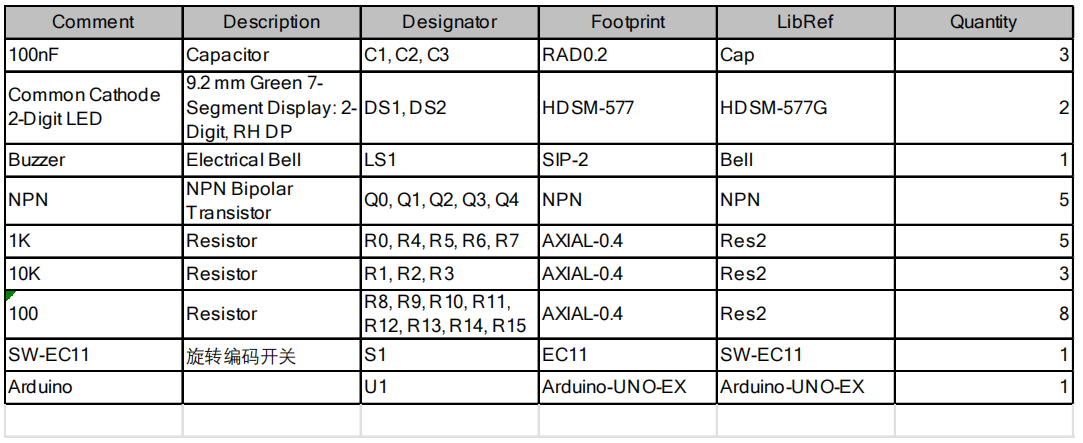
\includegraphics[width=0.95\textwidth]{bom.png}
  \caption{A4 倒计时定时器主要元器件清单截图}
  \label{fig:bom-image}
\end{figure}

\begin{table}[H]
  \centering
  \caption{关键元器件功能分组与选型依据}
  \label{tab:bom}
  \begin{tabular}{>{\raggedright\arraybackslash}p{0.16\textwidth}
                  >{\raggedright\arraybackslash}p{0.34\textwidth}
                  >{\raggedright\arraybackslash}p{0.38\textwidth}}
    \toprule
    功能模块 & 元器件与取值 & 选型依据 \\
    \midrule
    显示器件 & DS1、DS2：HDSM-577G 共阴 2 位 LED & 满足四位 MMSS 显示，符合实验共阴要求 \\
    段限流 & R8--R15：$100\,\Omega$ & 限制动态扫描峰值段电流 \\
    位选驱动 & Q1--Q4：NPN，R4--R7：$1\,\mathrm{k}\Omega$ & 四个公共阴极分时接地 \\
    报警驱动 & LS1 蜂鸣器，Q0：NPN，R0：$1\,\mathrm{k}\Omega$ & 提高报警负载驱动能力并保护 I/O \\
    编码输入 & S1：SW-EC11，R1--R3：$10\,\mathrm{k}\Omega$ & A/B 相上拉与按键状态检测 \\
    抗干扰 & C1--C3：$100\,\mathrm{nF}$ & 输入抖动与局部高频噪声抑制 \\
    主控接口 & U1：Arduino-UNO-EX & 与 Arduino UNO 引脚兼容，便于扩展板插接 \\
    \bottomrule
  \end{tabular}
\end{table}

\makepart{软件逻辑设计与程序实现}

\subsection*{1. 状态机与时间数组}

软件采用停止设定和倒计时运行两个主状态。停止状态下，旋转编码器每检测到一个有效步进，时间数组索引 \texttt{selectedTimeIndex} 加一或减一，并将数组中的 BCD 风格数值换算为分钟和秒；按下编码器按键后，变量 \texttt{stopped} 翻转，系统进入倒计时运行状态。运行状态下，程序依据 \texttt{millis()} 判断是否经过 $1000\,\mathrm{ms}$，若未到零则递减一秒；若中途再次按下编码器按键，则 \texttt{stopped} 重新置为停止状态，当前 \texttt{timerMinute} 与 \texttt{timerSecond} 保持不变，因此可以暂停在例如 $14\,\mathrm{s}$ 的中间状态。

倒计时到 $00:00$ 后，程序调用 \texttt{playMelody()}，通过 \texttt{tone()} 函数依次输出一组音符频率，使蜂鸣器播放一段提示旋律。与单一长鸣相比，旋律报警更容易被识别，也便于在调试时判断程序是否真正进入了计时结束分支。

\subsection*{2. 编码器软件消抖}

旋转编码器机械触点在切换瞬间会产生数毫秒抖动，若直接把每一次电平变化都当作有效步进，会出现跳数或反向误判。本程序保存上一次 A、B 相状态，并在 A 相由低电平变为高电平时结合 B 相电平判断旋转方向；上电后的前 $300\,\mathrm{ms}$ 内，程序暂不响应编码器输入，避免 Arduino 复位和 I/O 初始化阶段产生误步进。硬件上的 C1、C2 与上拉电阻共同抑制触点抖动，软件边沿判定则进一步减少重复计数。

\subsection*{3. 数码管动态扫描与 EEPROM 记忆}

动态扫描逻辑的核心是分时轮流点亮四位数码管。对共阴极电路，段选高电平有效，位选高电平使对应 NPN 管饱和导通；程序在 \texttt{updateDisplay()} 中把当前时间拆成四个十进制数字，依次调用 \texttt{setDigit()} 与 \texttt{setSegments()} 刷新显示。时间设定变化后，\texttt{changeSetTime()} 立即把 \texttt{selectedTimeIndex} 写入 EEPROM；因此将 Arduino 断电后再上电，程序能读回上次设定的时间索引，恢复常用倒计时设置。

本次联调使用的 Arduino 程序见附录代码 \ref{lst:core-code}。代码中保留了实际下载测试所用的引脚映射、倒计时数组、旋律报警和 EEPROM 记忆逻辑。

从程序结构看，\texttt{loop()} 并不是简单地等待某一个事件，而是在显示刷新过程中持续调用 \texttt{process()}。这样既能保持数码管动态扫描的刷新频率，又能在显示间隙读取编码器、处理暂停和更新倒计时。由于 \texttt{EEPROM.write()} 只在设定时间变化时调用，正常倒计时过程中不会频繁擦写 EEPROM，能够满足本实验对掉电记忆的要求。

\makepart{PCB 布线、制板、焊接与实验调试}

\subsection*{1. 本设计方案 PCB 版图与布线策略}

本设计阶段完成的 PCB 版图如图 \ref{fig:pcb-layout} 所示。板卡以 Arduino UNO 扩展板排针为边界约束，显示模块布置在下方中央，旋转编码器与蜂鸣器位于上方操作区，便于用户旋钮设定和听取报警。段线与位选线数量较多，因此 PCB 采用双层走线：红色顶层和蓝色底层交替跨越，以减少跳线并保持 Arduino 排针到数码管的连接可追踪。

\begin{figure}[H]
  \centering
  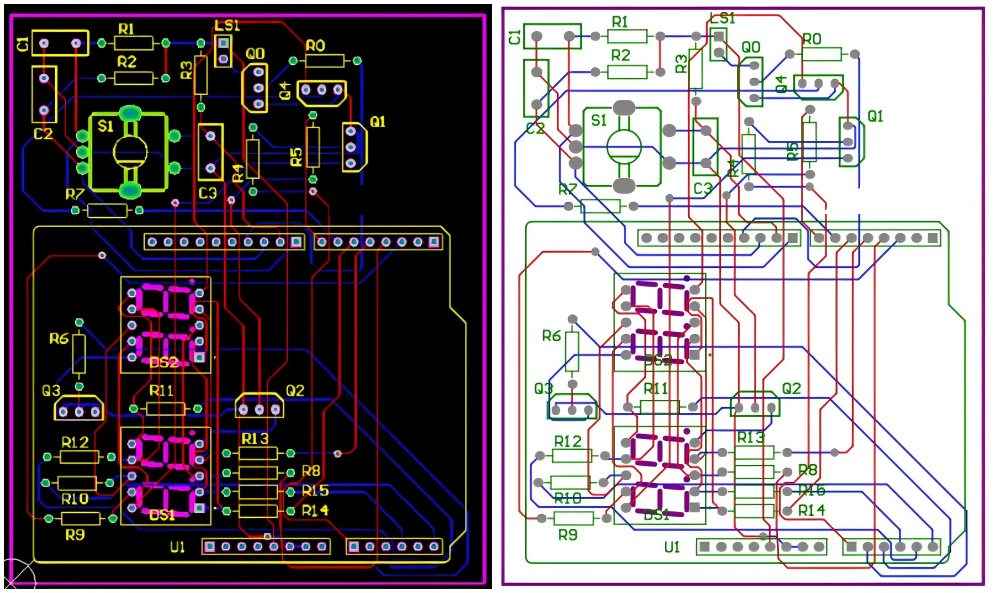
\includegraphics[width=0.96\textwidth]{pcb_layout.png}
  \caption{本设计方案的 A4 倒计时定时器双层 PCB 版图与丝印布局}
  \label{fig:pcb-layout}
\end{figure}

布线时应重点处理三类网络。第一，$5\,\mathrm{V}$ 与 GND 为整板公共参考，应尽可能采用较宽走线或铺铜连接，降低显示扫描和蜂鸣器动作引起的公共阻抗耦合。第二，C1--C3 等 $100\,\mathrm{nF}$ 电容应靠近编码器触点和输入节点放置，使机械抖动与尖峰干扰在进入 Arduino 引脚前被旁路。第三，蜂鸣器支路和数码管位选支路存在相对较大的瞬时电流，应避免与编码器 A/B 相输入线长距离平行，以减小开关电流对输入判定的串扰。

从图 \ref{fig:pcb-layout} 可见，数码管段电阻集中布置在显示区两侧，便于调试时用万用表从 Arduino 引脚、限流电阻到 LED 段逐段追踪；Q0 与 LS1 靠近放置，缩短蜂鸣器电流回路，有助于降低开关噪声耦合面积。丝印中保留 R、Q、DS、LS 等器件编号，对焊接检查和故障定位较为有利。

AD 软件生成的三维装配图与 PCB 版图可共同用于焊接前检查，如图 \ref{fig:pcb-assembly} 所示。对于本设计方案，装配预览主要用于确认数码管、旋转编码器、蜂鸣器和 Arduino 排针之间没有明显空间干涉，同时检查丝印方向是否便于焊接和后续排查。实际焊接前若能先通过 3D 视图观察器件高度和排针位置，可减少因封装方向或器件间距判断失误造成的返工。

\begin{figure}[H]
  \centering
  \begin{subfigure}[t]{0.48\textwidth}
    \centering
    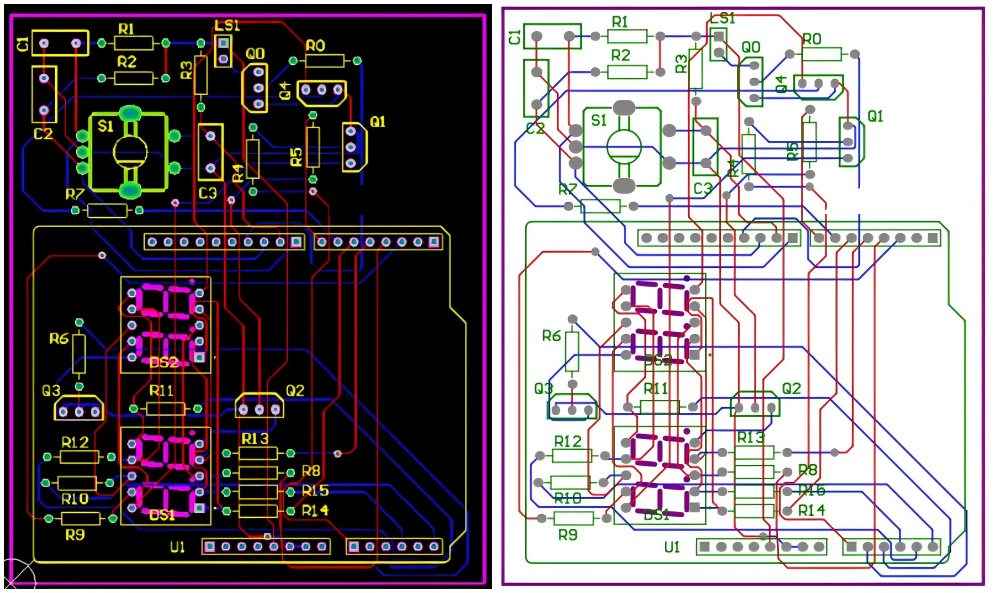
\includegraphics[width=\linewidth]{pcb_layout.png}
    \caption{PCB 版图用于检查走线与器件编号}
    \label{fig:pcb-layout-sub}
  \end{subfigure}
  \hfill
  \begin{subfigure}[t]{0.48\textwidth}
    \centering
    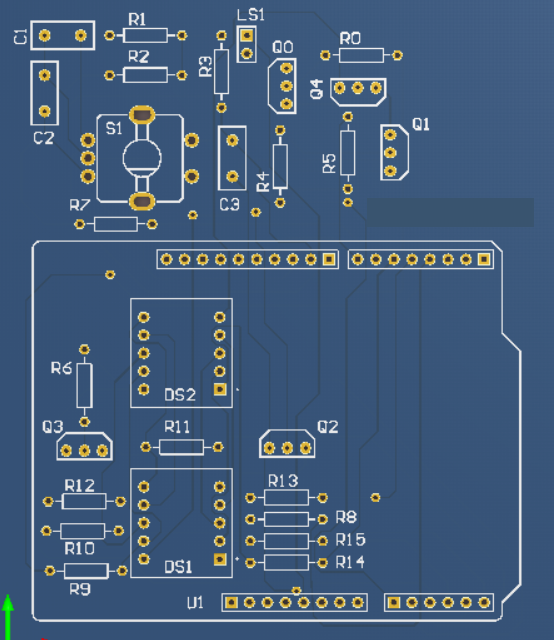
\includegraphics[width=0.82\linewidth]{pcb_3d.png}
    \caption{AD 3D 装配预览用于检查空间布局}
    \label{fig:pcb-3d-sub}
  \end{subfigure}
  \caption{本设计方案 PCB 版图与三维装配预览并排分析}
  \label{fig:pcb-assembly}
\end{figure}

参考电路图如图 \ref{fig:reference-circuit} 所示，可作为原始方案与本设计对照。相较于基础参考连接，本文设计在共阴极位选、段选有效电平和蜂鸣器 Q0 开关驱动方面进行了针对性调整。因此调试时不能直接套用共阳极段码取反逻辑，否则会出现显示全灭、显示反相或位选异常等现象。

\begin{figure}[H]
  \centering
  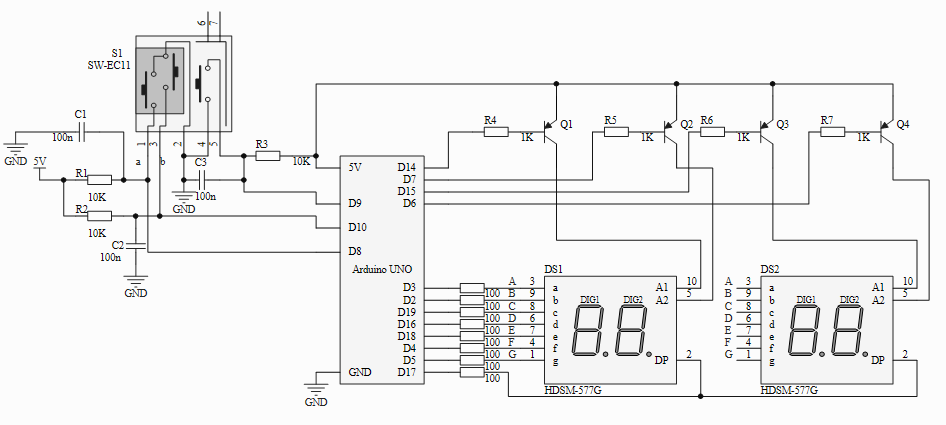
\includegraphics[width=0.96\textwidth]{reference_circuit.png}
  \caption{A4 倒计时定时器基础参考电路图与本设计方案对照依据}
  \label{fig:reference-circuit}
\end{figure}

联调流程可分为四步。首先进行静态电气检查，确认 $5\,\mathrm{V}$ 与 GND 无短路，数码管公共阴极没有误接到高电平总线；其次下载最小显示测试程序，逐位点亮 0--9，验证段序和位序是否与软件数组一致；再次加入编码器读取程序，观察顺时针与逆时针旋转是否对应时间索引增减，若方向相反可交换 A/B 判断或调整 \texttt{step} 符号；最后加入倒计时和报警逻辑，检查 $00:01\rightarrow00:00$ 过程中显示、蜂鸣器和状态切换是否同步。本次实物调试正是在这一流程基础上展开。

\subsection*{2. 实际制板方案与 PCB 布线观察}

前文已完成倒计时定时器的系统方案、硬件电路、软件逻辑和 PCB 布线分析。实际制板阶段，小组内需要统一提交一套 PCB 文件进行加工，经组内比较后最终采用同组同学的制板方案。该方案与本文分析的系统框架一致，均由 Arduino UNO、旋转编码器、四位共阴极数码管、蜂鸣器报警和 EEPROM 记忆构成，因此本文的实物实验以实际制成板为对象，对焊接质量和功能实现进行验证。

实际制板使用的原理图与 PCB 版图如图 \ref{fig:fabricated-design} 所示。板卡以 Arduino UNO 排针为接口边界，右侧布置两片双位数码管，左侧布置旋转编码器和去抖电容，中部集中放置段限流电阻、位选三极管和蜂鸣器驱动三极管。红色与蓝色走线分别表示双层 PCB 的顶层和底层连接，数码管段线数量较多，因此需要通过双层交叉布线降低跳线需求。

\begin{figure}[H]
  \centering
  \begin{subfigure}[t]{0.48\textwidth}
    \centering
    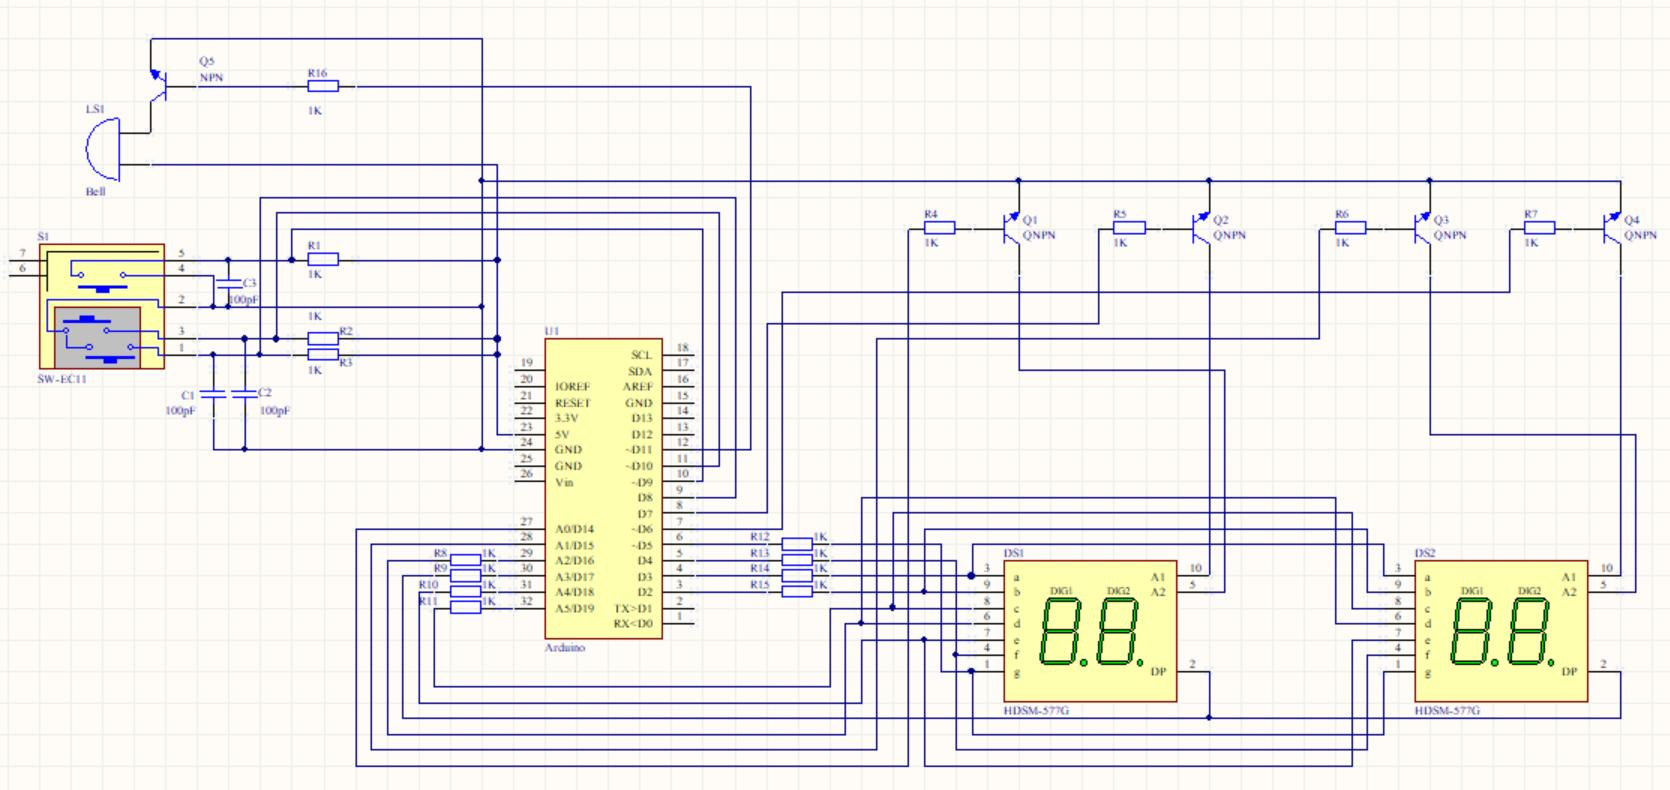
\includegraphics[width=\linewidth]{fabricated_schematic.png}
    \caption{制板采用的完整原理图}
    \label{fig:fabricated-schematic}
  \end{subfigure}
  \hfill
  \begin{subfigure}[t]{0.48\textwidth}
    \centering
    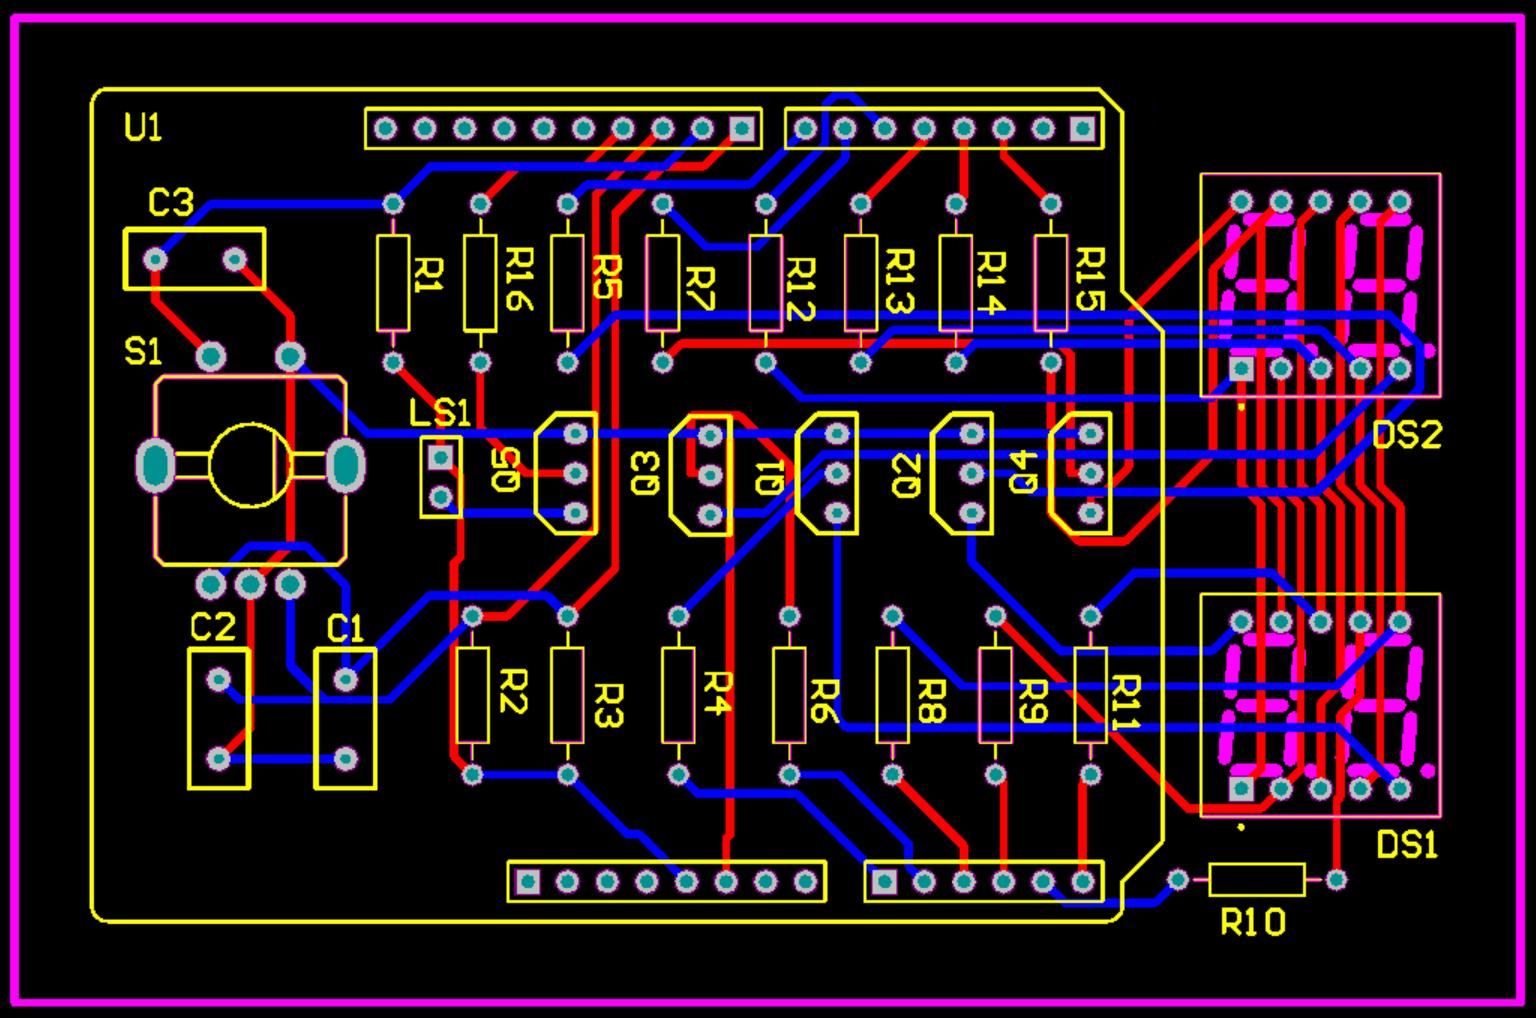
\includegraphics[width=\linewidth]{fabricated_pcb_layout.png}
    \caption{制板采用的双层 PCB 版图}
    \label{fig:fabricated-pcb}
  \end{subfigure}
  \caption{A4 倒计时定时器实际制板方案}
  \label{fig:fabricated-design}
\end{figure}

布线时应重点处理三类网络。第一，$5\,\mathrm{V}$ 与 GND 为整板公共参考，应尽可能采用较宽走线或铺铜连接，降低显示扫描和蜂鸣器动作引起的公共阻抗耦合。第二，C1--C3 等 $100\,\mathrm{nF}$ 电容应靠近编码器触点和输入节点放置，使机械抖动与尖峰干扰在进入 Arduino 引脚前被旁路。第三，蜂鸣器支路和数码管位选支路存在相对较大的瞬时电流，应避免与编码器 A/B 相输入线长距离平行，以减小开关电流对输入判定的串扰。

从图 \ref{fig:fabricated-pcb} 可见，数码管段电阻集中布置在显示区附近，便于调试时用万用表从 Arduino 引脚、限流电阻到 LED 段逐段追踪；蜂鸣器驱动管与 LS1 接口靠近放置，缩短报警电流回路，有助于降低开关噪声耦合面积。丝印中保留 R、Q、DS、LS 等器件编号，对焊接检查和故障定位较为有利。

\subsection*{3. 焊接装配与静态检查}

完成 PCB 加工后，按照从低矮器件到高大器件的顺序焊接：先焊接电阻和瓷片电容，再焊接三极管、Arduino 排针、旋转编码器和数码管。焊接完成后的正面与背面如图 \ref{fig:soldered-board} 所示。正面可观察到电阻阵列、三极管方向、编码器和数码管安装位置；背面则重点检查排针焊点、数码管焊盘和相邻焊点之间是否存在锡桥。

\begin{figure}[H]
  \centering
  \begin{subfigure}[t]{0.48\textwidth}
    \centering
    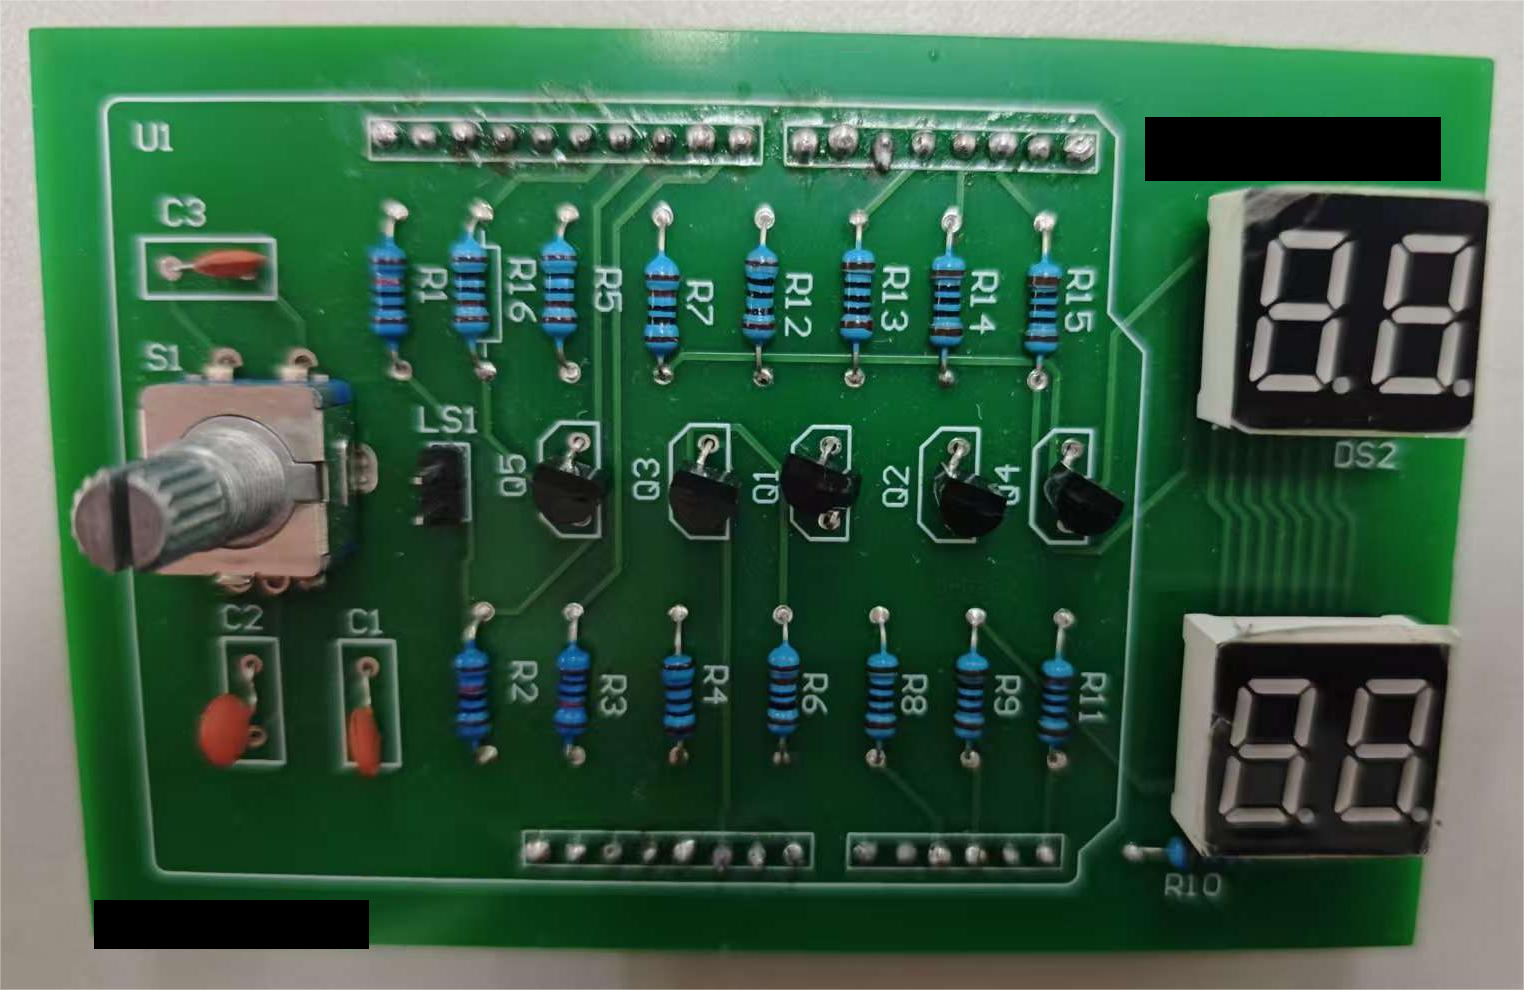
\includegraphics[width=\linewidth]{../实物照片/焊接正面.png}
    \caption{焊接完成后的 PCB 正面}
    \label{fig:solder-front}
  \end{subfigure}
  \hfill
  \begin{subfigure}[t]{0.48\textwidth}
    \centering
    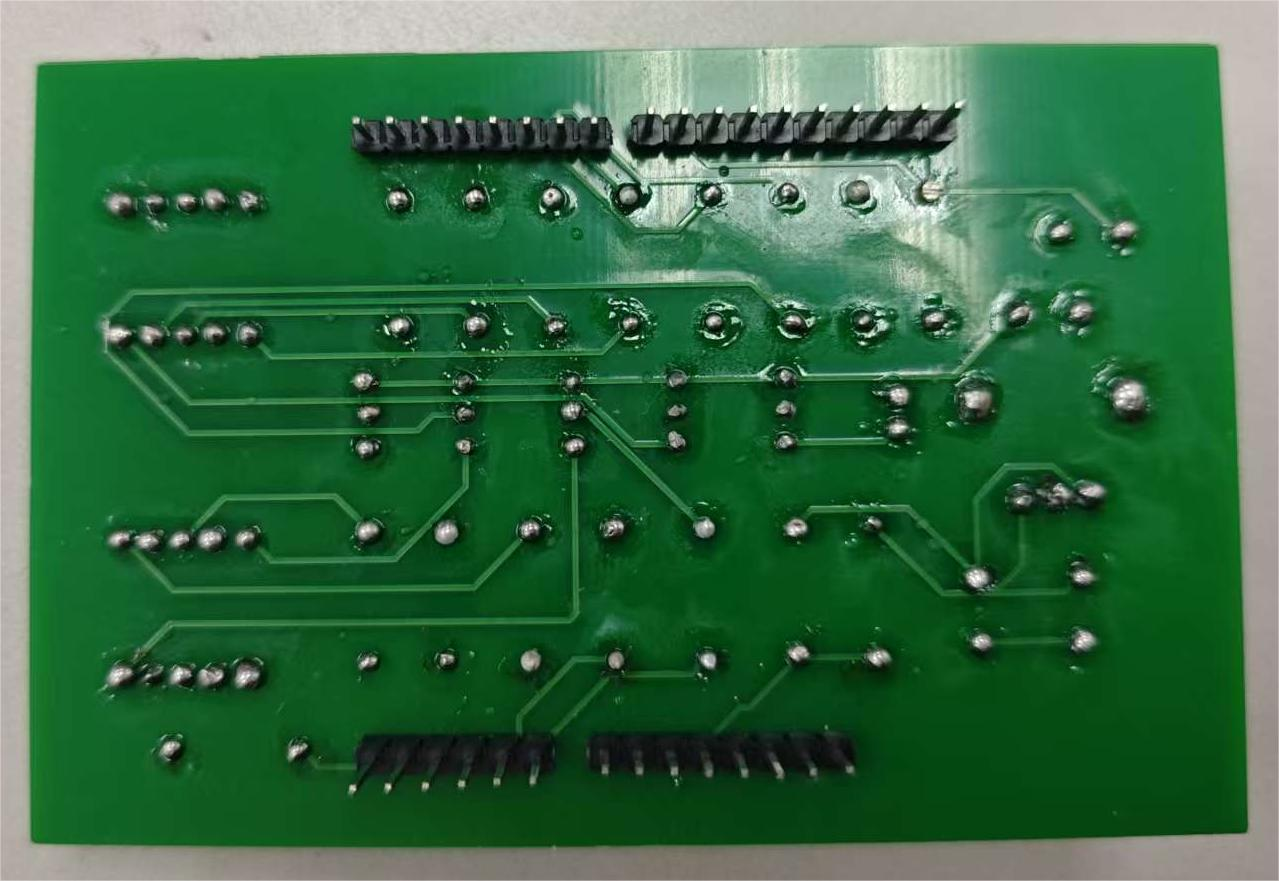
\includegraphics[width=\linewidth]{../实物照片/焊接背面.png}
    \caption{焊接完成后的 PCB 背面}
    \label{fig:solder-back}
  \end{subfigure}
  \caption{A4 倒计时定时器实物焊接检查}
  \label{fig:soldered-board}
\end{figure}

上电前先使用万用表电阻挡检查 $5\,\mathrm{V}$ 与 GND 之间无短路，并逐一观察数码管排针、Arduino 排针和三极管焊盘是否有虚焊。由于显示模块和报警支路都存在瞬时电流，若电源与地之间存在锡桥，通电后可能直接造成 Arduino 或 USB 供电端口过流，因此静态检查是实物调试前最重要的一步。

\subsection*{4. 上电测试与功能验证}

通过 Arduino UNO 给扩展板供电并下载程序后，数码管能够稳定显示预设时间，上电效果如图 \ref{fig:power-on} 所示。图中显示为 $00:05$，说明四位数码管的位选、段选以及动态扫描逻辑均已工作。蜂鸣器在本次测试中通过引线接入 LS1 对应位置，便于观察和听辨倒计时结束时的旋律报警。

\begin{figure}[H]
  \centering
  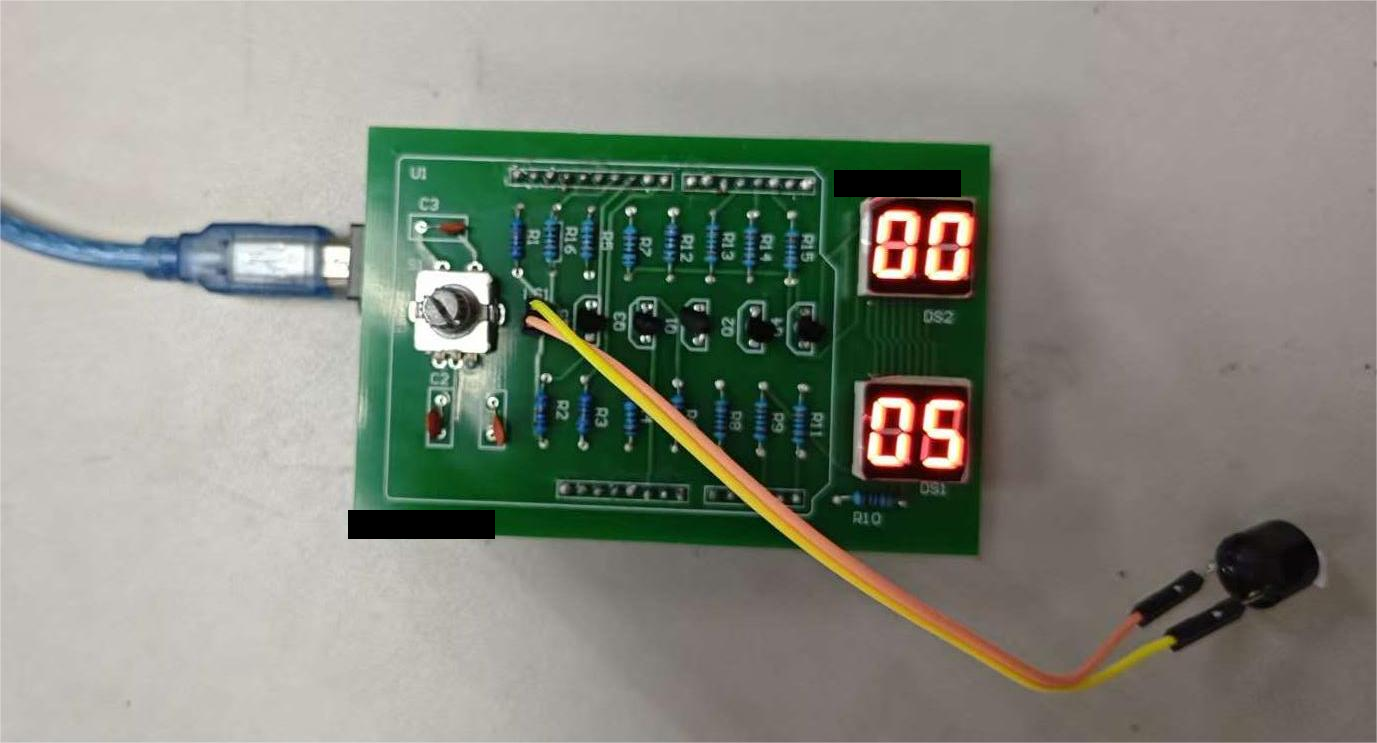
\includegraphics[width=0.78\textwidth]{../实物照片/上电测试.png}
  \caption{A4 倒计时定时器上电显示 $00:05$ 的实物效果}
  \label{fig:power-on}
\end{figure}

\begin{table}[H]
  \centering
  \caption{A4 倒计时定时器实物功能测试记录}
  \label{tab:test-result}
  \begin{tabular}{>{\raggedright\arraybackslash}p{0.19\textwidth}
                  >{\raggedright\arraybackslash}p{0.30\textwidth}
                  >{\raggedright\arraybackslash}p{0.38\textwidth}}
    \toprule
    测试项目 & 操作方法 & 测试现象与结论 \\
    \midrule
    旋钮设定 & 停止状态下旋转编码器 & 显示时间随旋转方向在预设数组中增减，说明 A/B 相方向判定有效 \\
    启动倒计时 & 按下旋转编码器开关 & 数码管按秒递减，显示无明显闪烁，状态切换正常 \\
    中途暂停 & 倒计时过程中再次按下编码器 & 计时停止并保持当前显示，例如可暂停在 $14\,\mathrm{s}$ 左右，说明状态保持逻辑有效 \\
    终点报警 & 倒计时归零 & 蜂鸣器播放一段旋律，说明 D11 输出、Q0 开关驱动和蜂鸣器支路工作正常 \\
    掉电记忆 & 设定某一时间后断电再上电 & 上电后恢复上次设定时间，说明 EEPROM 中的时间索引保存有效 \\
    \bottomrule
  \end{tabular}
\end{table}

\makepart{实验结果、误差分析与故障排查}

制板前根据原理图和 PCB 检查结果，预期系统能够形成倒计时定时器的基本功能闭环：编码器提供设定输入，Arduino UNO 完成状态控制和计时，四位共阴极数码管显示 MMSS，EEPROM 保存时间索引，蜂鸣器由 Q0 开关支路驱动。综合表 \ref{tab:test-result} 的功能测试结果可知，实物板已经验证了上述预期：旋转编码器能够改变设定时间，按下编码器可启动倒计时，再次按下可暂停并保持当前显示，倒计时归零后蜂鸣器能够播放旋律报警，断电后重新上电能够恢复上次设定时间。由此说明主控程序、数码管动态扫描、编码器输入、EEPROM 记忆和蜂鸣器驱动均已完成基本验证。

第一，时间误差主要来自 Arduino UNO 的时钟频率偏差以及程序中显示扫描、旋律播放等阻塞过程。由于本次实验以功能验证为主，未使用高精度秒表进行长时间计时误差统计；从短时间倒计时观察看，秒级递减节奏正常，能够满足课程实验对倒计时功能的要求。若后续需要定量评价，可分别设定 $30\,\mathrm{s}$、$60\,\mathrm{s}$、$300\,\mathrm{s}$ 等时间，用秒表记录实际结束时刻并计算相对误差。

第二，显示效果主要受动态扫描频率、段限流电阻和数码管本身亮度一致性的影响。实物上电后，四位显示能稳定呈现 $00:05$ 等时间数值，未观察到影响读数的明显重影。若出现某一位偏暗或缺段，应优先检查对应位选三极管、段限流电阻和数码管焊点，再检查程序中的位选顺序和段码表。

第三，编码器输入的主要风险是机械抖动导致跳数。实测旋转编码器能够正确改变设定时间，说明硬件电容去抖与软件边沿检测能够满足本次实验。若快速旋转时出现漏计或方向偶发错误，可进一步采用完整四状态格雷码译码，或在 A/B 相输入端加入施密特触发整形。

第四，报警支路的排查重点是 Q0 开关驱动和蜂鸣器类型。实测倒计时结束时能够播放旋律，说明 Arduino D11 端口输出、基极电阻、Q0 导通以及蜂鸣器连接均有效。若后续出现声音弱或不响，应按 D11 输出波形、Q0 集电极电压、蜂鸣器极性和焊点连通性依次排查。

\makepart{思考题与拓展讨论}

\subsection*{1. 定时加热控制的实现思路}

倒计时定时器可扩展为定时加热控制器。由于加热器通常工作在较高电压和较大电流下，不能由 Arduino I/O 直接驱动。可将蜂鸣器输出逻辑扩展为继电器、MOSFET 或固态继电器驱动：Arduino 输出经光耦或三极管驱动继电器线圈，继电器触点串接在加热器供电回路中。为提高安全性，交流负载应加入保险丝、压敏电阻或 RC 吸收网络，并保证强电和弱电 PCB 间距满足绝缘要求。

\subsection*{2. 消除秒钟滴答声的方法}

本程序中每秒更新倒计时时会短暂拉高蜂鸣器形成滴答提示声。若希望只在倒计时结束时报警，可删除每秒递减过程中的短脉冲蜂鸣器控制，仅保留归零后的旋律或终点判断：
\[
  \text{buzzer}= 
  \begin{cases}
    1, & \text{timerMinute}=0\ \text{且}\ \text{timerSecond}=0,\\
    0, & \text{其他情况}.
  \end{cases}
\]
这样蜂鸣器只在终点状态发声，不再随每秒节拍产生提示音。若需要静音倒计时和结束短鸣兼顾，可增加报警持续时间变量，例如归零后蜂鸣 $3\,\mathrm{s}$ 自动关闭。

\makepart{实验总结与体会}

本实验完成了 A4 倒计时定时器从方案分析、原理图理解、PCB 制板、元器件焊接到 Arduino 程序联调的完整过程。系统以 Arduino UNO 为主控，采用旋转编码器进行时间设定，两片共阴极 2 位 7 段 LED 进行动态扫描显示，并通过 EEPROM 实现上电恢复上次设定时间。实物测试表明，旋钮设定、按键启动、倒计时中途暂停、归零旋律报警和掉电记忆等功能均能正常实现。

从硬件角度看，本实验进一步加深了对共阴极数码管动态扫描和三极管开关驱动的理解。数码管显示是否正确，不仅取决于段码表，还取决于位选管导通逻辑、公共端连接方式和焊接质量；蜂鸣器能否可靠发声，也不仅是程序输出高低电平的问题，还与 Q0 的基极驱动、集电极回路和蜂鸣器类型有关。通过实物焊接与上电排查，可以更直观地认识到原理图符号、PCB 封装和真实器件方向之间必须一一对应。

从软件角度看，旋转编码器读取、动态扫描刷新、倒计时节拍和 EEPROM 写入需要在同一个主循环中协调。若显示刷新阻塞过长，会影响按键响应和计时精度；若 EEPROM 写入位置不合理，则可能造成不必要的擦写。最终程序采用状态变量 \texttt{stopped} 区分设定、运行和暂停行为，并在设定时间变化时保存索引，使功能逻辑较为清晰。后续若继续完善，可增加更精确的计时误差测试、长时间稳定性测试和外壳结构设计，使该倒计时定时器更接近可长期使用的小型电子产品。

\clearpage
\appendix
\section*{附录：Arduino 实测程序}
\addcontentsline{toc}{section}{附录：Arduino 实测程序}

\lstinputlisting[caption={A4 倒计时定时器 Arduino 实测程序},label={lst:core-code}]{../程序/CountdownTimer/CountdownTimer.ino}

\end{document}
